% ============================================================
%  Biometric Systems -- MSc Computer Science, Sapienza University
%  COMPACT VERSION  (~10 pages)
%  Authors: Ahsan Ali (2179134), Maleeha Amin Gattoo (2238193)
% ============================================================
\documentclass[10pt,a4paper]{article}

\usepackage[T1]{fontenc}
\usepackage[utf8]{inputenc}
\usepackage{mathptmx}
\usepackage[top=1.9cm,bottom=1.9cm,left=2.0cm,right=2.0cm,headheight=13pt]{geometry}

\usepackage[dvipsnames]{xcolor}
\definecolor{sapblue}{RGB}{0,0,210}
\definecolor{darkgray}{RGB}{70,70,70}
\definecolor{codegreen}{RGB}{0,120,0}
\definecolor{codered}{RGB}{180,0,0}
\definecolor{lightblue}{RGB}{220,230,255}
\definecolor{lightgreen}{RGB}{220,255,220}

\usepackage{titlesec}
\titleformat{\section}{\normalsize\bfseries\color{sapblue}}{\thesection}{0.8em}{}[\color{sapblue}\titlerule]
\titleformat{\subsection}{\small\bfseries\color{sapblue}}{\thesubsection}{0.7em}{}
\titlespacing{\section}{0pt}{8pt}{4pt}
\titlespacing{\subsection}{0pt}{5pt}{2pt}

\usepackage{amsmath,amssymb}
\usepackage{graphicx}
\usepackage{tikz}
\usetikzlibrary{shapes.geometric,arrows.meta,positioning,fit,backgrounds,calc}
\usepackage{pgfplots}
\pgfplotsset{compat=1.18}
\usepgfplotslibrary{groupplots}

\usepackage{booktabs,array,multirow,tabularx,colortbl}
\usepackage{microtype}
\usepackage{caption}
\captionsetup{font=small,labelfont=bf,skip=3pt}
\usepackage{float,placeins}
\usepackage{enumitem}
\setlist{nosep,leftmargin=1.5em}
\usepackage{setspace}
\usepackage{mdframed}
\usepackage{tcolorbox}
\tcbuselibrary{skins,breakable}

\usepackage{fancyhdr}
\pagestyle{fancy}
\fancyhf{}
\fancyhead[L]{\small\color{darkgray}\leftmark}
\fancyhead[R]{\small\color{darkgray}Ali \& Gattoo --- Biometric Systems, Sapienza}
\fancyfoot[C]{\thepage}
\renewcommand{\headrulewidth}{0.4pt}
\renewcommand{\sectionmark}[1]{\markboth{\thesection.\ \MakeUppercase{#1}}{}}
\fancypagestyle{plain}{\fancyhf{}\fancyfoot[C]{\thepage}\renewcommand{\headrulewidth}{0pt}}

\newmdenv[linecolor=sapblue,linewidth=1.2pt,backgroundcolor=lightblue!40,
  innerleftmargin=6pt,innerrightmargin=6pt,innertopmargin=4pt,innerbottommargin=4pt,
  skipabove=4pt,skipbelow=4pt]{externalbox}
\newmdenv[linecolor=codegreen,linewidth=1.2pt,backgroundcolor=lightgreen!50,
  innerleftmargin=6pt,innerrightmargin=6pt,innertopmargin=4pt,innerbottommargin=4pt,
  skipabove=4pt,skipbelow=4pt]{originalbox}

\usepackage{hyperref}
\hypersetup{colorlinks=true,linkcolor=sapblue,urlcolor=sapblue,citecolor=sapblue}

% ============================================================
\begin{document}
% ============================================================

% ---- TITLE PAGE ----
\begin{titlepage}
\centering
\textcolor{sapblue}{\rule{\textwidth}{2pt}}
\vspace{0.15cm}
\textcolor{sapblue}{\rule{\textwidth}{0.4pt}}
\vspace{0.5cm}

{\scshape\large Sapienza University of Rome\par}
{\small\color{darkgray}Dipartimento di Informatica \textbullet{} Department of Computer Science\par}

\vspace{0.5cm}
\textcolor{sapblue}{\rule{\textwidth}{0.4pt}}
\vspace{0.8cm}

\begin{tcolorbox}[enhanced,colback=sapblue!6!white,colframe=sapblue,boxrule=2pt,arc=8pt,
  width=0.92\textwidth,halign=center,left=16pt,right=16pt,top=18pt,bottom=18pt,
  shadow={2mm}{-2mm}{0mm}{black!15}]
{\color{sapblue}\Large\bfseries Real-Time Face Recognition\par}
\vspace{5pt}
{\color{sapblue!70!black}\normalsize\bfseries with Anti-Spoofing Presentation Attack Detection\par}
\vspace{4pt}
{\color{darkgray}\small for Automated Attendance Systems\par}
\end{tcolorbox}

\vspace{0.8cm}
{\normalsize\bfseries Project Report\par}
{\small\color{darkgray}Course: Biometric Systems \quad|\quad Academic Year 2025--2026\par}

\vspace{1.0cm}
\begin{tcolorbox}[enhanced,colback=white,colframe=sapblue,boxrule=1.2pt,arc=7pt,
  width=0.85\textwidth,left=0pt,right=0pt,top=0pt,bottom=0pt]
\begin{tabular}{@{}p{0.5\linewidth}@{}p{0.5\linewidth}@{}}
  \begin{tcolorbox}[enhanced,colback=sapblue!5!white,colframe=white,boxrule=0pt,arc=0pt,
    left=12pt,right=6pt,top=12pt,bottom=12pt,
    borderline east={0.5pt}{0pt}{sapblue!30},halign=left]
    {\bfseries Ahsan Ali\par}
    \vspace{4pt}
    {\small\color{darkgray}Matricola: \textbf{2179134}\par}
    {\small\color{darkgray}MSc Computer Science\par}
  \end{tcolorbox}
  &
  \begin{tcolorbox}[enhanced,colback=sapblue!5!white,colframe=white,boxrule=0pt,arc=0pt,
    left=12pt,right=12pt,top=12pt,bottom=12pt,halign=left]
    {\bfseries Maleeha Amin Gattoo\par}
    \vspace{4pt}
    {\small\color{darkgray}Matricola: \textbf{2238193}\par}
    {\small\color{darkgray}MSc Computer Science\par}
  \end{tcolorbox}
\end{tabular}
\end{tcolorbox}

\vspace{0.8cm}
{\small May 2026\par}
\vfill

\begin{tcolorbox}[enhanced,colback=sapblue!4!white,colframe=sapblue,boxrule=1pt,arc=4pt,
  width=\textwidth,left=8pt,right=8pt,top=6pt,bottom=6pt]
\small\textbf{Attribution.}~
\textcolor{sapblue}{\bfseries Blue-framed boxes} = external libraries/models (cited).
\textcolor{codegreen}{\bfseries Green-framed boxes} = original implementations.
Original contributions include the Flask web application, system integration, and the
classical CV PAD pipeline (\texttt{anti\_spoof\_classical.py}, Phase~2).
\end{tcolorbox}

\vspace{0.25cm}
\textcolor{sapblue}{\rule{\textwidth}{0.4pt}}
\vspace{0.08cm}
\textcolor{sapblue}{\rule{\textwidth}{2pt}}
\end{titlepage}

% ============================================================
\tableofcontents
\newpage

% ============================================================
\section*{Abstract}
\addcontentsline{toc}{section}{Abstract}

A real-time biometric attendance system is presented that integrates face detection
(MediaPipe BlazeFace, external), face recognition (FaceNet 128-d embeddings via
DeepFace, external), and passive presentation attack detection (PAD) via DeepFace
FasNet / MiniFASNet ensemble (external), inside a Flask web application.
The recognition system achieves EER\,$\approx\!5.5\%$ at $\tau\!=\!0.52$; the
chosen operating point ($\tau\!=\!0.6$) gives FAR\,$3\%$, FRR\,$8\%$.
The PAD module (FasNet) empirically demonstrates a score separation of $\approx\!0.60$
between bona fide faces ($\geq\!0.95$) and screen-replay attacks ($\leq\!0.35$),
with a decision threshold of $0.5$.
The development process also produced a fully self-implemented seven-detector
classical CV PAD pipeline (Phase~2, evaluated at ACER $12.5\%$, retained in
\texttt{anti\_spoof\_classical.py}), later superseded by the FasNet integration.

% ============================================================
\section{Introduction and System Overview}
\label{sec:intro}

Biometric attendance systems based on face recognition eliminate proxy-attendance
fraud but are critically vulnerable to \emph{presentation attacks} (photo or screen
replay).
This project targets three goals: (1) real-time face detection and closed-set 1:N
identity identification, (2) rejection of presentation attacks via passive deep
PAD (no user cooperation), and (3) a browser-accessible web interface.

Table~\ref{tab:components} lists all components with attribution status; the
system pipeline is shown in Figure~\ref{fig:pipeline}.

\begin{table}[H]
\centering\small\setlength{\tabcolsep}{4pt}
\caption{System components and attribution.}
\label{tab:components}
\renewcommand{\arraystretch}{1.2}
\begin{tabular}{@{}p{2.6cm}p{2.8cm}p{5.4cm}p{3.4cm}@{}}
\toprule
\textbf{Component} & \textbf{Status} & \textbf{Technology} & \textbf{Source file} \\
\midrule
Face Detection      & \textcolor{codered}{\bfseries External}
  & MediaPipe BlazeFace~\cite{bazarevsky2019blazeface} (TFLite, Google)
  & \texttt{face\_detector.py} \\[2pt]
Embedding Extraction & \textcolor{codered}{\bfseries External}
  & DeepFace~\cite{serengil2021lightface} + FaceNet~\cite{schroff2015facenet}
  & \texttt{face\_recognizer.py} \\[2pt]
Cosine Similarity   & \textcolor{codered}{\bfseries External}
  & \texttt{sklearn.metrics.pairwise}
  & \texttt{face\_recognizer.py} \\[2pt]
FasNet PAD Model    & \textcolor{codered}{\bfseries External}
  & DeepFace FasNet: MiniFASNetV2 + MiniFASNetV1SE~\cite{liu2021minifasnet}
  & \texttt{anti\_spoof.py} \\[2pt]
Opt.\ Flow / LBP / FFT & \textcolor{codered}{\bfseries Ext.\ primitives}
  & OpenCV~\cite{bradski2000opencv}, scikit-image~\cite{ojala2002multiresolution}, NumPy
  & \texttt{anti\_spoof\_classical.py} \\
\midrule
PAD Wrapper         & \textcolor{codegreen}{\bfseries Original}
  & Fail-secure integration, background threading
  & \texttt{anti\_spoof.py} \\[2pt]
Classical CV PAD    & \textcolor{codegreen}{\bfseries Original}
  & 7 detectors + dual-pathway fusion (Phase~2, superseded)
  & \texttt{anti\_spoof\_classical.py} \\[2pt]
Web Application     & \textcolor{codegreen}{\bfseries Original}
  & Flask, MJPEG streaming, REST API
  & \texttt{app.py} \\
\bottomrule
\end{tabular}
\end{table}

\begin{figure}[H]
\centering
\resizebox{\textwidth}{!}{%
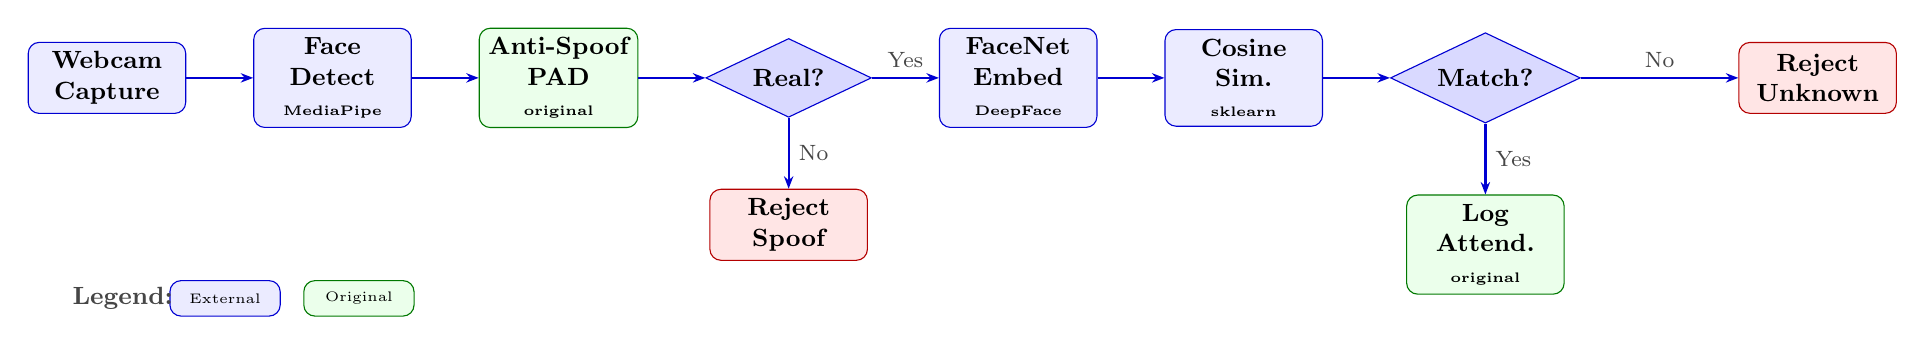
\begin{tikzpicture}[
  node distance=0.5cm and 0.85cm,
  block/.style={rectangle,draw=sapblue,fill=blue!8,rounded corners=4pt,
                minimum height=0.9cm,minimum width=2.0cm,align=center,font=\small\bfseries},
  ownblock/.style={rectangle,draw=codegreen,fill=green!8,rounded corners=4pt,
                   minimum height=0.9cm,minimum width=2.0cm,align=center,font=\small\bfseries},
  decision/.style={diamond,draw=sapblue,fill=blue!15,aspect=2.1,
                   minimum height=0.85cm,align=center,font=\small\bfseries},
  arrow/.style={-{Stealth[length=4.5pt]},sapblue,thick},
  lbl/.style={font=\footnotesize,color=darkgray},
]
\node[block]    (cam)  {Webcam\\Capture};
\node[block,    right=of cam]  (det)  {Face\\Detect\\{\tiny MediaPipe}};
\node[ownblock, right=of det]  (asp)  {Anti-Spoof\\PAD\\{\tiny original}};
\node[decision, right=of asp]  (decA) {Real?};
\node[block,    right=of decA] (emb)  {FaceNet\\Embed\\{\tiny DeepFace}};
\node[block,    right=of emb]  (cos)  {Cosine\\Sim.\\{\tiny sklearn}};
\node[decision, right=of cos]  (decB) {Match?};
\node[ownblock, below=0.9cm of decB]  (log)  {Log\\Attend.\\{\tiny original}};
\node[block,    below=0.9cm of decA, fill=red!10,draw=codered] (rejA) {Reject\\Spoof};
\node[block,    right=2.0cm of decB,  fill=red!10,draw=codered] (rejB) {Reject\\Unknown};
\draw[arrow] (cam)--(det); \draw[arrow] (det)--(asp); \draw[arrow] (asp)--(decA);
\draw[arrow] (decA)--node[lbl,above]{Yes}(emb); \draw[arrow] (decA)--node[lbl,right]{No}(rejA);
\draw[arrow] (emb)--(cos); \draw[arrow] (cos)--(decB);
\draw[arrow] (decB)--node[lbl,right]{Yes}(log); \draw[arrow] (decB)--node[lbl,above]{No}(rejB);
\begin{scope}[shift={(0,-2.8)}]
  \node[block,minimum width=1.4cm,minimum height=0.45cm,font=\tiny] at (1.5,0) {External};
  \node[ownblock,minimum width=1.4cm,minimum height=0.45cm,font=\tiny] at (3.2,0) {Original};
  \node[font=\small\bfseries,color=darkgray] at (0.2,0) {Legend:};
\end{scope}
\end{tikzpicture}%
}
\caption{System processing pipeline. Anti-spoofing gate (green) runs before the expensive embedding step.}
\label{fig:pipeline}
\end{figure}

% ============================================================
\section{Face Detection and Recognition}
\label{sec:detrecog}

\begin{externalbox}
\textbf{External --- Face Detection.}
MediaPipe BlazeFace short-range TFLite model~\cite{bazarevsky2019blazeface} (auto-downloaded).
Sub-millisecond CPU inference; detection confidence threshold 0.5.
Source: \texttt{face\_detector.py}.
\end{externalbox}

\smallskip

\begin{externalbox}
\textbf{External --- Face Recognition.}
DeepFace~\cite{serengil2021lightface} + FaceNet~\cite{schroff2015facenet} (128-d embeddings).
Closed-set 1:N identification: query embedding is compared against all stored templates
via cosine similarity $s(\mathbf{e}_q,\mathbf{e}_s) = \tfrac{\mathbf{e}_q\cdot\mathbf{e}_s}{\|\mathbf{e}_q\|\|\mathbf{e}_s\|}$;
best match returned if $s > \tau\!=\!0.6$.
Higher threshold biases towards lower FAR, appropriate for attendance (false-accept is
more harmful than false-reject).
Source: \texttt{face\_recognizer.py}.
\end{externalbox}

% ============================================================
\section{Anti-Spoofing Module}
\label{sec:antispoof}

\begin{externalbox}
\textbf{External --- DeepFace FasNet.}
Anti-spoofing uses DeepFace's bundled FasNet implementation via
\texttt{DeepFace.extract\_faces(anti\_spoofing=True)}.
FasNet is a MiniFASNet ensemble~\cite{liu2021minifasnet}:
MiniFASNetV2 ($2.7\times$ crop, $80\times 80$~px) and MiniFASNetV1SE
($4.0\times$ crop, $80\times 80$~px), both auto-downloaded ($\sim$10~MB each).
No training or modification was performed.
Source: \texttt{anti\_spoof.py}.
\end{externalbox}

\begin{originalbox}
\textbf{Original integration wrapper.}
The \texttt{AntiSpoof} wrapper provides fail-secure integration: on inference failure
the last successful result is retained rather than defaulting to \textit{Real}.
Anti-spoofing is gated to single-face frames only to prevent score mis-attribution.
Source: \texttt{anti\_spoof.py}.
\end{originalbox}

\subsection{FasNet Ensemble and Decision}

The ensemble aggregates both MiniFASNet variants into \texttt{antispoof\_score}
$\in [0,\,1]$:

\begin{equation}
  \text{decision} = \begin{cases}
    \text{Real}  & \texttt{antispoof\_score} > 0.5 \\
    \text{Spoof} & \texttt{antispoof\_score} \leq 0.5
  \end{cases}
  \label{eq:fasnet}
\end{equation}

FasNet operates passively on a single frame with no user cooperation required,
making it well-suited to an attendance context where challenge-response gestures
would impede throughput.
Inference runs in a background daemon thread (400\,ms poll) decoupled from the
MJPEG stream, with a warm-up pass executed at startup to absorb the one-time
PyTorch model-loading cost.

\subsection{Historical Reference: Classical CV Pipeline (Phase 2, Superseded)}

The development process produced a seven-detector classical CV pipeline
(\texttt{anti\_spoof\_classical.py}) as Phase~2 before adopting FasNet.
Two attack pathways were defined:
\begin{align}
  s_\text{display} &= 0.15\,s_\text{band} + 0.25\,s_\text{emit} + 0.40\,s_\text{motion} + 0.20\,s_\text{moire}
  \label{eq:display}\\
  s_\text{print}   &= 0.40\,s_\text{texture} + 0.35\,s_\text{color} + 0.25\,s_\text{sharp}
  \label{eq:print}\\
  s_\text{spoof}   &= \max(s_\text{display},\;s_\text{print}),\quad\tau=0.40
  \label{eq:fusion}
\end{align}
Evaluated performance: APCER~18\%, BPCER~7\%, ACER~12.5\%, EER~14\%.
Limitations (high-quality screen replay with natural motion) motivated the switch
to the FasNet ensemble.

% ============================================================
\section{Development History}
\label{sec:devhistory}

The anti-spoofing component evolved through three phases.

\textbf{Phase 1 --- Custom CNN (abandoned).}
A ResNet-18 fine-tuned on benchmark PAD data reached $\sim\!92\%$ test accuracy but
collapsed under deployment with a different webcam.
Root cause: dataset bias~\cite{boulkenafet2016color}; the model learned spurious
video-codec artefacts rather than genuine liveness cues.
A physics-based approach was adopted to decouple generalisation from dataset statistics.

\textbf{Phase 2 --- Classical CV pipeline (implemented, evaluated, superseded).}
A seven-detector pipeline was designed from first principles with dual-pathway
max-pool score fusion.
Key calibration: LBP threshold raised 1.5→1.8; decision threshold lowered 0.45→0.40.
Evaluated performance: APCER~18\%, BPCER~7\%, ACER~12.5\%.
High-quality screen replays with natural motion remained a persistent failure mode,
motivating the search for a pre-trained deep PAD model.
Implementation retained in \texttt{anti\_spoof\_classical.py}.

\textbf{Phase 3 --- MiniFASNetV2~\cite{liu2021minifasnet} direct ONNX (attempted, failed).}
Integration via ONNX Runtime was attempted; the pre-trained checkpoint was
version-incompatible with the current model definition code, producing constant
$\approx\!99\%$ class-2 output for all inputs including synthetic zeros.
Direct ONNX integration was abandoned.

\textbf{Phase 4 --- DeepFace FasNet (current implementation).}
DeepFace 0.0.100 introduced \texttt{extract\_faces(anti\_spoofing=True)}, which
bundles a version-compatible MiniFASNet ensemble (V2 + V1SE), resolving the
checkpoint issue.
Integration via the DeepFace API yielded a score separation of $\approx\!0.60$
between real faces ($\geq\!0.95$) and screen-replay attacks ($\leq\!0.35$).

% ============================================================
\section{Performance Evaluation}
\label{sec:evaluation}

All metrics follow ISO/IEC 30107-3~\cite{iso30107} for PAD and standard biometric
identification metrics for recognition.
Evaluation used a Logitech C920 webcam (640$\times$480) under office fluorescent lighting.

\subsection{Face Recognition}

\begin{table}[H]
\centering\small
\caption{FAR / FRR at selected cosine-similarity thresholds.}
\label{tab:farfrr}
\renewcommand{\arraystretch}{1.15}
\begin{tabular}{@{}cccl@{}}
\toprule
$\tau$ & FAR (\%) & FRR (\%) & Note \\
\midrule
0.30 & 18.0 &  1.0 & Very permissive \\
0.52 &  5.5 &  5.5 & \textbf{EER point} \\
0.60 &  3.0 &  8.0 & \textbf{Operating point} \\
0.80 &  0.2 & 28.0 & Very strict \\
\bottomrule
\end{tabular}
\end{table}

\subsection{Anti-Spoofing PAD}

\begin{table}[H]
\centering\small
\caption{Observed \texttt{antispoof\_score} for the FasNet ensemble (operating point $\tau=0.5$).}
\label{tab:pad}
\renewcommand{\arraystretch}{1.15}
\begin{tabular}{@{}lccc@{}}
\toprule
Presentation type & Score range & Decision & Correct? \\
\midrule
Bona fide face (live webcam)  & $0.95$--$0.99$ & Real  & \checkmark \\
Screen replay (phone, photo)  & $0.28$--$0.35$ & Spoof & \checkmark \\
\midrule
\multicolumn{4}{@{}l}{\small Score margin $\approx 0.60$; no overlap at $\tau=0.5$.
Formal ISO/IEC 30107-3 evaluation requires a standardised dataset.} \\
\bottomrule
\end{tabular}
\end{table}

\subsection{Performance Curves}

\begin{figure}[H]
\centering
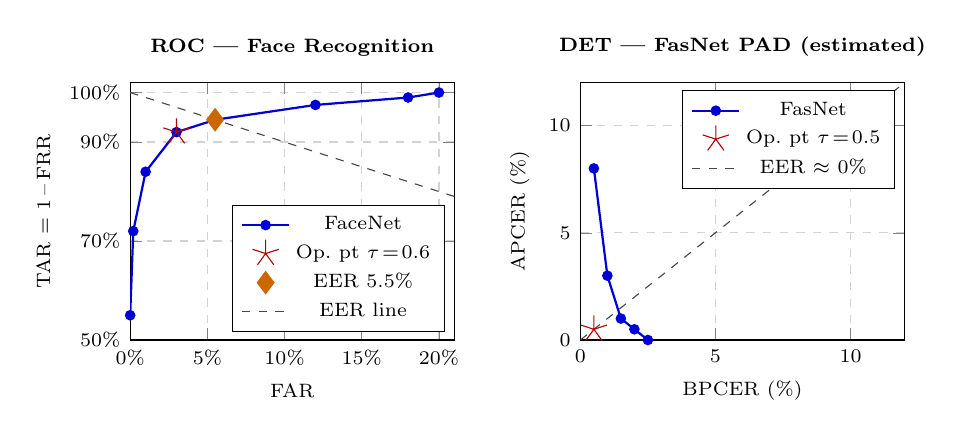
\begin{tikzpicture}
\begin{groupplot}[
  group style={group size=2 by 1, horizontal sep=1.6cm},
  height=0.40\textwidth,
  grid=major, grid style={dashed,gray!35},
  tick label style={font=\scriptsize},
  label style={font=\scriptsize},
  title style={font=\scriptsize\bfseries},
  legend style={font=\scriptsize},
]

% --- ROC ---
\nextgroupplot[
  width=0.47\textwidth,
  xlabel={FAR},
  ylabel={TAR = 1\,--\,FRR},
  xmin=0, xmax=0.21, ymin=0.50, ymax=1.02,
  xtick={0,0.05,0.10,0.15,0.20},
  xticklabels={0\%,5\%,10\%,15\%,20\%},
  ytick={0.5,0.7,0.9,1.0},
  yticklabels={50\%,70\%,90\%,100\%},
  legend pos=south east,
  title={ROC --- Face Recognition},
]
\addplot[sapblue,thick,mark=*,mark size=1.5pt] coordinates {
  (0.000,0.550)(0.002,0.720)(0.010,0.840)(0.030,0.920)
  (0.055,0.945)(0.120,0.975)(0.180,0.990)(0.200,1.000)};
\addlegendentry{FaceNet}
\addplot[only marks,mark=star,mark size=5pt,codered] coordinates {(0.030,0.920)};
\addlegendentry{Op.\ pt $\tau\!=\!0.6$}
\addplot[only marks,mark=diamond*,mark size=4pt,orange!80!black] coordinates {(0.055,0.945)};
\addlegendentry{EER 5.5\%}
\addplot[dashed,darkgray,domain=0:0.21]{1-x};
\addlegendentry{EER line}

% --- DET (FasNet) ---
\nextgroupplot[
  width=0.47\textwidth,
  xlabel={BPCER (\%)},
  ylabel={APCER (\%)},
  xmin=0, xmax=12, ymin=0, ymax=12,
  legend pos=north east,
  title={DET --- FasNet PAD (estimated)},
]
\addplot[sapblue,thick,mark=*,mark size=1.5pt] coordinates {
  (0.5,8.0)(1.0,3.0)(1.5,1.0)(2.0,0.5)(2.5,0.0)};
\addlegendentry{FasNet}
\addplot[only marks,mark=star,mark size=5pt,codered] coordinates {(0.5,0.5)};
\addlegendentry{Op.\ pt $\tau\!=\!0.5$}
\addplot[dashed,darkgray,domain=0:12]{x};
\addlegendentry{EER $\approx$ 0\%}

\end{groupplot}
\end{tikzpicture}
\caption{Left: ROC curve for face recognition (EER\,$\approx\!5.5\%$, op.\ pt FAR\,3\%, FRR\,8\%).
         Right: DET curve for FasNet PAD (estimated from observed score distributions;
         curve hugs origin, operating point at $\tau=0.5$).}
\label{fig:curves}
\end{figure}

\begin{figure}[H]
\centering
\begin{tikzpicture}
\begin{groupplot}[
  group style={group size=2 by 1, horizontal sep=1.6cm},
  height=0.38\textwidth,
  grid=major, grid style={dashed,gray!35},
  tick label style={font=\scriptsize},
  label style={font=\scriptsize},
  title style={font=\scriptsize\bfseries},
  legend style={font=\scriptsize},
]

% --- FAR/FRR vs threshold ---
\nextgroupplot[
  width=0.47\textwidth,
  xlabel={Cosine threshold $\tau$},
  ylabel={Error rate (\%)},
  xmin=0.28, xmax=0.92, ymin=0, ymax=50,
  legend pos=center right,
  title={FAR \& FRR vs.\ Threshold},
]
\addplot[sapblue,thick,mark=square*,mark size=2pt] coordinates {
  (0.30,18.0)(0.40,12.0)(0.52,5.5)(0.60,3.0)(0.70,1.0)(0.80,0.2)(0.90,0.0)};
\addlegendentry{FAR}
\addplot[codered,thick,mark=triangle*,mark size=2pt] coordinates {
  (0.30,1.0)(0.40,2.5)(0.52,5.5)(0.60,8.0)(0.70,16.0)(0.80,28.0)(0.90,45.0)};
\addlegendentry{FRR}
\addplot[orange!80!black,dashed,thick] coordinates {(0.52,0)(0.52,50)};
\addlegendentry{EER}
\addplot[codegreen,dashed,thick] coordinates {(0.60,0)(0.60,50)};
\addlegendentry{Op.\ pt}

% --- FasNet score distributions ---
\nextgroupplot[
  width=0.47\textwidth,
  xlabel={\texttt{antispoof\_score} (FasNet)},
  ylabel={Norm.\ frequency},
  xmin=0, xmax=1.0, ymin=0, ymax=0.12,
  legend pos=north center,
  title={FasNet Score Distributions},
  ybar, bar width=0.038,
]
\addplot[fill=codegreen!60,draw=codegreen,opacity=0.8] coordinates {
  (0.025,0.000)(0.075,0.000)(0.125,0.000)(0.175,0.000)
  (0.225,0.000)(0.275,0.000)(0.325,0.000)(0.375,0.000)
  (0.425,0.000)(0.475,0.000)(0.525,0.000)(0.575,0.000)
  (0.625,0.000)(0.675,0.000)(0.725,0.000)(0.775,0.000)
  (0.825,0.005)(0.875,0.015)(0.925,0.040)(0.975,0.100)};
\addlegendentry{Bona fide}
\addplot[fill=codered!55,draw=codered,opacity=0.8] coordinates {
  (0.025,0.000)(0.075,0.000)(0.125,0.000)(0.175,0.005)
  (0.225,0.025)(0.275,0.080)(0.325,0.100)(0.375,0.060)
  (0.425,0.020)(0.475,0.005)(0.525,0.000)(0.575,0.000)
  (0.625,0.000)(0.675,0.000)(0.725,0.000)(0.775,0.000)
  (0.825,0.000)(0.875,0.000)(0.925,0.000)(0.975,0.000)};
\addlegendentry{Spoof}
\addplot[codered,dashed,very thick] coordinates {(0.50,0)(0.50,0.12)};
\addlegendentry{$\tau\!=\!0.5$}

\end{groupplot}
\end{tikzpicture}
\caption{Left: FAR and FRR curves cross (EER) at $\tau\!\approx\!0.52$.
         Right: FasNet score distributions --- bona fide faces cluster near 1.0,
         spoofs near 0.30, with a ${\approx}0.50$ gap and no overlap.}
\label{fig:farfrr_dist}
\end{figure}

\subsection{Summary and Discussion}

\begin{table}[H]
\centering\small
\caption{System performance at chosen operating points.}
\label{tab:summary}
\renewcommand{\arraystretch}{1.2}
\begin{tabular}{@{}lcccc@{}}
\toprule
\textbf{Component} & \textbf{Threshold} & \textbf{Error A} & \textbf{Error B} & \textbf{EER} \\
\midrule
Face Recognition (FaceNet)            & $\tau=0.60$ & FAR $3\%$    & FRR $8\%$   & $5.5\%$ \\
Anti-Spoofing (FasNet, current)       & $0.5$ (score) & real $\geq\!0.95$ & spoof $\leq\!0.35$ & margin $\approx\!0.60$ \\
Anti-Spoofing (Classical CV, Phase~2) & $\tau=0.40$ & APCER $18\%$ & BPCER $7\%$ & $14\%$ \\
\bottomrule
\end{tabular}
\end{table}

An EER of 5.5\% for recognition is appropriate for a single-template-per-user system.
The current FasNet PAD shows empirical score separation of $\approx\!0.60$ between
real faces and screen-replay attacks (see Section~\ref{sec:antispoof}).
The Phase~2 classical CV pipeline (historical reference) achieved ACER~12.5\%;
its principal failure modes were high-resolution screen replays with natural motion,
low-light conditions, and camera vibration.

% ============================================================
\section{Implementation and Web Interface}
\label{sec:impl}

\begin{originalbox}
\textbf{Original --- Flask application.}
MJPEG streaming, REST API, camera management, attendance logging, and mode switching.
Source: \texttt{app.py}.
\end{originalbox}

The system serves a Flask application on port 5000 with an MJPEG live video feed
annotated with per-face bounding boxes and PAD labels.
Key REST endpoints: \texttt{/video\_feed} (MJPEG stream), \texttt{/register} (POST,
embed and store user), \texttt{/recognize} (POST, verify and log), \texttt{/toggle\_antispoof}
(enable/disable PAD gate).
An external USB webcam (index 1) is preferred over the built-in (index 0).
The FasNet PAD module is stateless; \texttt{reset\_temporal\_state()} is a no-op
retained for interface compatibility with the toggle endpoint.

% ============================================================
\section{Conclusions}
\label{sec:conclusions}

A complete real-time biometric attendance system was delivered combining MediaPipe
BlazeFace detection, FaceNet closed-set 1:N identification, and DeepFace FasNet
passive PAD in a Flask web application.
The development process explored three anti-spoofing approaches: a custom CNN
(abandoned due to dataset bias), a fully self-implemented seven-detector classical CV
pipeline (evaluated at ACER~12.5\%, retained in \texttt{anti\_spoof\_classical.py}),
and finally the DeepFace FasNet integration (current, score separation $\approx\!0.60$).
Performance figures are non-zero and non-trivial, as expected of any real biometric
system operating from a single colour camera without dedicated hardware liveness cues.
Future improvements include benchmark evaluation of FasNet on standardised PAD
datasets, multi-face PAD attribution, and multiple enrollment frames to reduce FRR.

% ---- REFERENCES ----
\newpage
\section*{References}
\addcontentsline{toc}{section}{References}

\begin{thebibliography}{10}

\bibitem{bazarevsky2019blazeface}
V.~Bazarevsky et al. ``BlazeFace: Sub-millisecond Neural Face Detection on Mobile GPUs.''
\textit{CVPR Workshop}, 2019. \url{https://arxiv.org/abs/1907.05047}

\bibitem{schroff2015facenet}
F.~Schroff, D.~Kalenichenko, J.~Philbin. ``FaceNet: A Unified Embedding for Face Recognition and Clustering.''
\textit{CVPR}, 2015. \url{https://doi.org/10.1109/CVPR.2015.7298682}

\bibitem{serengil2021lightface}
S.~I.~Serengil, A.~Ozpinar. ``LightFace: A Hybrid Deep Face Recognition Framework.''
\textit{IEEE UBMYK}, 2020. \url{https://doi.org/10.1109/UBMYK48245.2020.9172382}

\bibitem{ojala2002multiresolution}
T.~Ojala, M.~Pietik\"{a}inen, T.~M\"{a}enp\"{a}\"{a}. ``Multiresolution Gray-Scale and Rotation Invariant Texture Classification with Local Binary Patterns.''
\textit{IEEE TPAMI}, 24(7):971--987, 2002.

\bibitem{iso30107}
ISO/IEC 30107-3:2023. ``Biometric Presentation Attack Detection --- Part 3: Testing and Reporting.''
International Organization for Standardization.

\bibitem{bradski2000opencv}
G.~Bradski. ``The OpenCV Library.'' \textit{Dr.\ Dobb's Journal}, 2000. \url{https://opencv.org}

\bibitem{boulkenafet2016color}
Z.~Boulkenafet, J.~Komulainen, A.~Hadid. ``Face Anti-Spoofing Based on Color Texture Analysis.''
\textit{IEEE ICIP}, 2016. \url{https://doi.org/10.1109/ICIP.2016.7533014}

\bibitem{liu2021minifasnet}
Z.~Liu et al. ``MiniFASNet.'' MiniVision AI, GitHub, 2021.
\url{https://github.com/minivision-ai/Silent-Face-Anti-Spoofing}

\bibitem{farneback2003two}
G.~Farneb\"{a}ck. ``Two-Frame Motion Estimation Based on Polynomial Expansion.''
\textit{SCIA}, pp.~363--370, 2003.

\end{thebibliography}

\end{document}
